\documentclass[10pt]{article}

\usepackage{sectsty}
\usepackage{graphicx}
\usepackage[T1]{fontenc}
\usepackage{epigraph} %quotes
\usepackage{amssymb} %math symbols
\usepackage{mathtools} %more math stuff
\usepackage{amsmath}
\usepackage{amsfonts}
\usepackage{amsthm} %theorems, proofs and lemmas
\usepackage[font=small,labelfont=bf]{caption}
\usepackage{subcaption}
\usepackage[ruled,vlined]{algorithm2e} %algoritms/pseudocode
\usepackage{geometry}
\usepackage[dvipsnames]{xcolor}
\usepackage{fancyhdr}
\usepackage{tikz}
\usepackage{hyperref}

\usetikzlibrary{matrix,calc}

\geometry{
    a4paper,
    % total={190mm,257mm},
    left=20mm,
    right=20mm,
    top=20mm,
    bottom=20mm,
    }

%% Theorem notation
\newtheorem{theorem}{Theorem}[section]
\newtheorem{corollary}{Corollary}[theorem]
\newtheorem{lemma}[theorem]{Lemma}
\newtheorem{problem}{Problem}[section]

% \geometry{margin=1in}
%% declaring abs so that it works nicely
\DeclarePairedDelimiter\abs{\lvert}{\rvert}%
\DeclarePairedDelimiter\norm{\lVert}{\rVert}%


\pagestyle{fancy}
\fancyhf{}
\fancyhead[LE,RO]{EPFL – Spring Semester 2023}
\fancyhead[RE,LO]{Artificial neural networks/reinforcement learning (Gerstner)}
\rfoot{Page \thepage \hspace{1pt}} 
\renewcommand{\headrulewidth}{1pt}

% Swap the definition of \abs* and \norm*, so that \abs
% and \norm resizes the size of the brackets, and the 
% starred version does not.
\makeatletter
\let\oldabs\abs
\def\abs{\@ifstar{\oldabs}{\oldabs*}}
%
\let\oldnorm\norm
\def\norm{\@ifstar{\oldnorm}{\oldnorm*}}
\makeatother

\title{Mini-project 1: Deep Q-learning for Epidemic Mitigation}
\date{}

\begin{document}
\maketitle	
\thispagestyle{fancy}

\section{Introduction}

\subsection*{What is the project about?}

In this mini-project, you will train an artificial agent using deep-Q-learning to find a decision-making policy, regarding the mitigation of an epidemic process. You will compare performance of different methods with various \textbf{action} and \textbf{observation-spaces}.\\

% \noindent \textcolor{MidnightBlue}{\textbf{DELIVERABLES} : you will be ask to hand out the following documents: your source code, as well a jupyter notebook clearly showing how to reproduce your results and a \texttt{.pdf} file presenting your figues and your written answers (see the \LaTeX~  template in the project folder).}

\noindent
\textbf{What should you submit?}
\begin{enumerate}
  \item \textbf{Report} (in \texttt{.pdf} format):
  Report should be at most 10 pages. It should include the results of your analyses in answer to the questions below. Please do not elaborate over 1-3 sentences per (sub-)question. % Please respect the word limit for each question and choose a reasonable size for your figures.
  \item Jupyter notebook (in \texttt{.ipynb} format):
  The Jupyter notebook should contain the code for reproducing your results. The code should be well-documented and readable.

\end{enumerate}
\noindent
The report may be just a pdf version of the notebook, if you have answered the questions in the notebook. In this case,
make sure that it is clear what question is answered where; and also submit the notebook itself!

\noindent
\textbf{When should you submit?} \\
Either \textbf{A} Monday last week of teaching term, the 29th of May, or \textbf{B} Monday after end of teaching term, the 5th of June.
Choose your deadline yourself (\textbf{A} or \textbf{B}), but you must be available three days after your submission (\textbf{A}: May 31st or June 1st, \textbf{B}: June 6th or 7th) in
person for discussion of the miniproject (fraud detection interview).
\\



\subsection*{Working with the epidemic modeling environment}

\begin{figure}[h!]
  \centering
  \begin{subfigure}[t]{.47\textwidth}
    \centering
    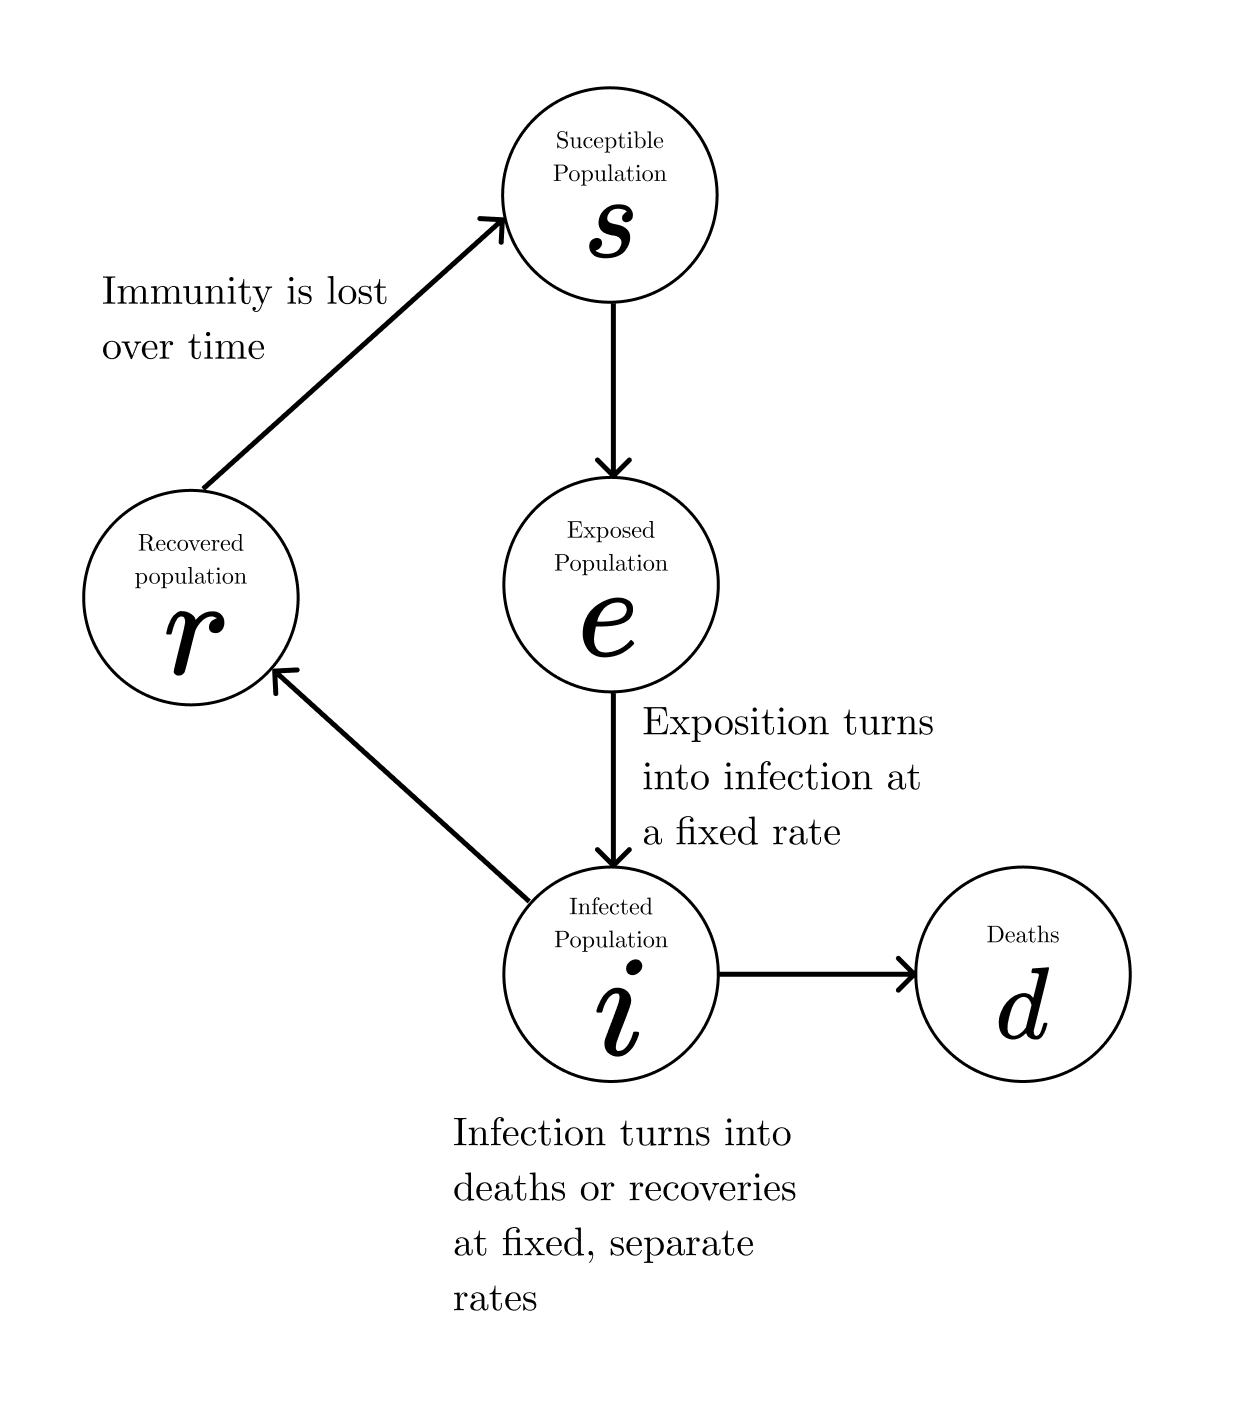
\includegraphics[width=.9\textwidth]{figures/seirds.png}
    \caption{Schematic representation of the flow of the state variables into each other in the epidemic model. Only \textbf{infected} and \textbf{deaths} are measurable.}
  \end{subfigure}%
  \hfill
  \begin{subfigure}[t]{.47\textwidth}
    \centering
    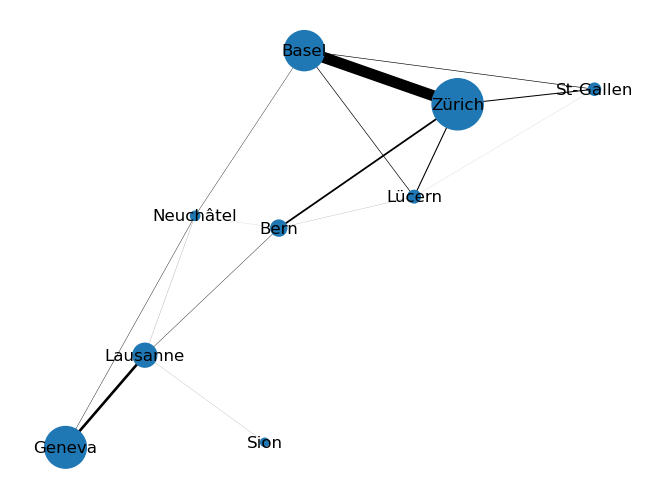
\includegraphics[width=.9\textwidth]{figures/switzerland.png}
    \caption{Approximate map of Switzerland. The size of the nodes is proportional to population; the width of the edges to the rate of cross-contamination between cities.}
  \end{subfigure}
  \caption{The environment dynamical model.}
  \label{fig:env}
\end{figure}


You will act as a computer scientist trying to provide insights for optimal decision making in the context of an epidemic scenario. 
An epidemic of a new virus named  \textit{MARVIN23} (apologies to any Marvin amongst the students) has just started
propagating in Switzerland's neighbor Listenburg. You will use a predictive model designed by epidemiologists to train
a reinforcement learning agent for \textit{epidemic mitigation}. The model takes the form of a few python classes that
we call a reinforcement learning \textit{environment}. It implements a simulation of epidemic dynamics on a simplified
map of Switzerland as well as a bunch of utility functions to facilitate RL implementation. \\

\subsubsection*{Simulating epidemics}

% Simulation Variables
The epidemic model is implemented through a set of stochastic differential equations with 5 simulation variables (see figure \ref{fig:env}a per-city on the map, drawn in figure \ref{fig:env}b). The variables represent susceptible ($s$), exposed ($e$), infected ($i$), recovered ($r$) and dead ($d$) individuals (see table \ref{table:states} for details), and each variable evolves in time following a set of differential equations.
% Time
Time in the simulation is measured in \textit{days}, since the onset of the epidemic (which always happens on day $d_0=0$).
We denote time by the variable $d \in \mathbb{N}$. We use the superscript notation $\square^{(d)}$ to denote that a simulation variable is measured on day $d$, $s_\text{Lausanne}^{(17)}$ indicates the number of susceptible people in \textit{Lausanne}, $17$ days after the onset of the epidemic.
% Total Convention
We use the $\square_\text{total}$ convention to denote the total number of individuals in a given state across all cities, for instance, 
\begin{align*}
  s_\text{total}^{(d)} = \sum_{\text{city} \in \text{map}} s_\text{city}^{(d)},
\end{align*}
gives the total number of susceptible people in Switzerland on day $d$.

\begin{table}[ht]

  \begin{center}
    \begin{tabular}{||c | l ||} 
    \hline
    State variable & Quantity represented by the variable  \\ [0.5ex] 
    \hline\hline
    $s_\text{city}$ & number of \textit{susceptible} individuals in city "\textit{city}".  \\
    \hline
    $e_\text{city}$ & number of \textit{exposed} (infected but not yet contagious) individuals in city "\textit{city}". \\
    \hline
    $i_\text{city}$& number of \textit{infected} (and contagious) individuals in city "\textit{city}". \\
    \hline
    $r_\text{city}$ & number of \textit{recovered} (cannot be infected) individuals in city "\textit{city}".  \\
    \hline
    $d_\text{city}$ & number of \textit{dead} individuals in city "\textit{city}". \\ 
    \hline
    \end{tabular}
    \end{center}
    \caption{State variables of the dynamical model.}
    \label{table:states}
\end{table}

\subsubsection*{Decision Process}
In this project \textbf{we will implement agents which are only allowed to measure two of these variables}: $i_\text{city}$ and $d_\text{city}$ (for each city). The agent is also allowed to know the full population of each city at time $t=0$ (before the epidemic starts), which is useful to scale the parameters. 
This makes the problem we will later try to solve with reinforcement learning a control problem on \textbf{Partially Observable Markov Decision Processes} (\textit{POMDP}). The POMDP, uses a different time-step than the simulation, here, time is not measured in \textit{days} but rather in \textit{weeks}. 
In other words, the agent only makes one set of decisions per-week.  At each time step of the \textit{POMDP} the agent makes \textbf{observations} computes \textbf{actions} and a receives a \textbf{reward}. To avoid confusion between the simulation time-step measurements (in days) and the POMDP time-step measurements (in weeks) we use the following square brackets ($\square^{[w]}$) convention to denote a time-measurement in weeks and the parentheses convention ($\square^{(d)}$) to denote a measurement in days. 
Furthermore, we always assume that when we measure a simulation variable in weeks, that measurement is done \textit{on the last day of that week}. For instance notation $r_\text{Bern}^{[2]} = r_\text{Bern}^{(14)}$.


\begin{figure}[h!]
  \centering
  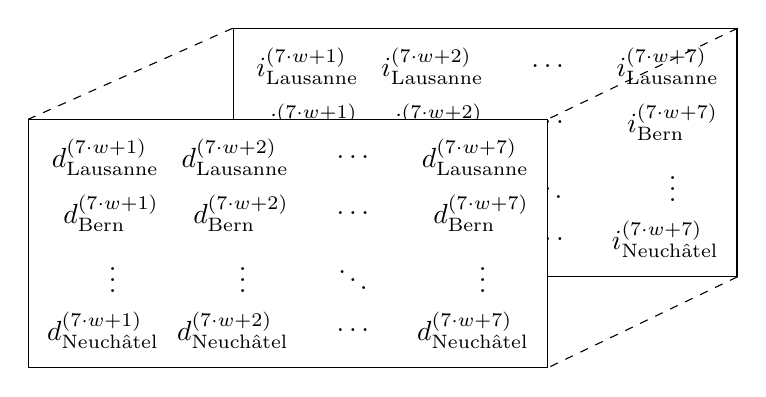
\begin{tikzpicture}[every node/.style={anchor=north east,fill=white,minimum width=1.4cm,minimum height=7mm}]
    \matrix (mA) [draw,matrix of math nodes]
    {
    i_\text{Lausanne}^{(7\cdot w + 1)} & i_\text{Lausanne}^{(7\cdot w + 2)} & \dots & i_\text{Lausanne}^{(7\cdot w+7)}  \\
    i_\text{Bern}^{(7\cdot w + 1 )} & i_\text{Bern}^{(7\cdot w + 2)} & \dots & i_\text{Bern}^{(7\cdot w+7)}  \\
    \vdots & \vdots & \ddots & \vdots \\
    i_\text{Neuchâtel}^{(7\cdot w + 1)} & i_\text{Neuchâtel}^{(7\cdot w + 2)} & \dots & i_\text{Neuchâtel}^{(7\cdot w+7)}  \\
    };
    
  
    \matrix (mC) [draw,matrix of math nodes] at ($(mA.south west)+(4.0,2.0)$)
    {
      d_\text{Lausanne}^{(7\cdot w + 1)} & d_\text{Lausanne}^{(7\cdot w + 2)} & \dots & d_\text{Lausanne}^{(7\cdot w+7)}  \\
      d_\text{Bern}^{(7\cdot w + 1)} & d_\text{Bern}^{(7\cdot w + 2)} & \dots & d_\text{Bern}^{(7\cdot w+7)}  \\
      \vdots & \vdots & \ddots & \vdots \\
      d_\text{Neuchâtel}^{(7\cdot w + 1)} & d_\text{Neuchâtel}^{(7\cdot w + 2)} & \dots & d_\text{Neuchâtel}^{(7\cdot w+7)}  \\
    };
    
    \draw[dashed](mA.north east)--(mC.north east);
    \draw[dashed](mA.north west)--(mC.north west);
    \draw[dashed](mA.south east)--(mC.south east);
    \end{tikzpicture}
  \caption{An example observation tensor measured on week $w$.}
  \label{fig:obs}
\end{figure}


\subsubsection*{Observations}

At each time step the agent receives an observation consisting in a measurement of the \textbf{number of infected} ($i_\text{city}^{(7\cdot w+d)}$) and \textbf{dead people}  ($d_\text{city}^{(7\cdot w+d)}$), in each city, on each day $i\in[0,...,6]$ of the week.
This gives an observation tensor $\mathbf{o}^{[w]} \in \mathbb{R}^{(2 \times 7 \times \text{\# cities})}$ (see figure \ref{fig:obs}). We call the set of all possible observations the \textbf{observation space} (denoted $O$).


The agent also has access to the total number of people in each city, before the epidemic started (this is meant to be used for scaling). Refer to the \textbf{tutorial jupyter notebook} (\texttt{tutorial.ipynb}) to learn how to actually gather observations using the environment library.

\subsubsection*{Actions}
The agent action space consists of $4$ binary decisions: \textbf{confinement}, \textbf{isolation}, \textbf{add additional hospital beds} and \textbf{vaccinate}. It is allowed for an agent to pick any combination of decisions, for instance: \textit{confine}, and \textit{vaccinate} but \textit{do not isolate}, and \textit{do not add additional hospital beds}. 
We denote the action taken by the agent on week $w$ as $\mathbf{a}^{[w]} \in \{\texttt{True},\texttt{False}\}^{4}$, we represent each decision as a boolean variable and thus the action is represented as a set of four labeled boolean variables. We use the convention that the action is \textit{being performed} when set to \texttt{True}. Actions can be written as composition of binary decisions as follows:

\begin{equation}
  \mathbf{a}^{[w]} = a_\textit{conf}^{[w]} \cup a_\text{isol}^{[w]} \cup a_\text{hosp}^{[w]} \cup a_\text{vacc}^{[w]} = \bigcup_{\mathfrak{d} \in \text{actions}}a_\mathfrak{d}^{[w]},
\end{equation}
where $a_\mathfrak{d}^{[w]} \in \{\texttt{True},\texttt{False}\}$ and $\mathfrak{d} \in [\text{conf},\text{isol},\text{hosp},\text{vacc}]$.
The effects of each decision is detailed in table \ref{table:actions}. Refer to the \textbf{tutorial jupyter notebook} to learn how to actually handle actions using the environment library. We call the set of all possible actions the \textbf{action space} (denoted $A$). All of the actions have an associated cost (see the \textbf{reward} paragraph).


\begin{table}[ht]
  \begin{center}
    \begin{tabular}{||l | l | l ||} 
     \hline
     notation & decision name & Effect  \\ [0.5ex] 
     \hline\hline
     $a_\text{conf}$ & \textbf{confinement} & Strongly reduces the rate at which  \\ 
      & & people are exposed to the virus.\\
     \hline
     $a_\text{isol}$ & \textbf{isolation} & Slows down propagation from one city to the next.  \\ 
      &  & Does not slows down exposition within a single city. \\ 
     \hline
     $a_\text{hosp}$ & \textbf{add hospital beds} & Reduces mortality. \\ 
      &  & Has no impact on the exposition/infection rate. \\ 
     \hline
     $a_\text{vacc}$ & \textbf{vaccinate} & Increases immunity directly. \\ 
      & &  Makes people recovered without them being infected.  \\ 
     \hline
    \end{tabular}
    \end{center}
    \caption{Actions and their exact effects.}
    \label{table:actions}
\end{table}

\begin{figure}[h!]
    \centering
    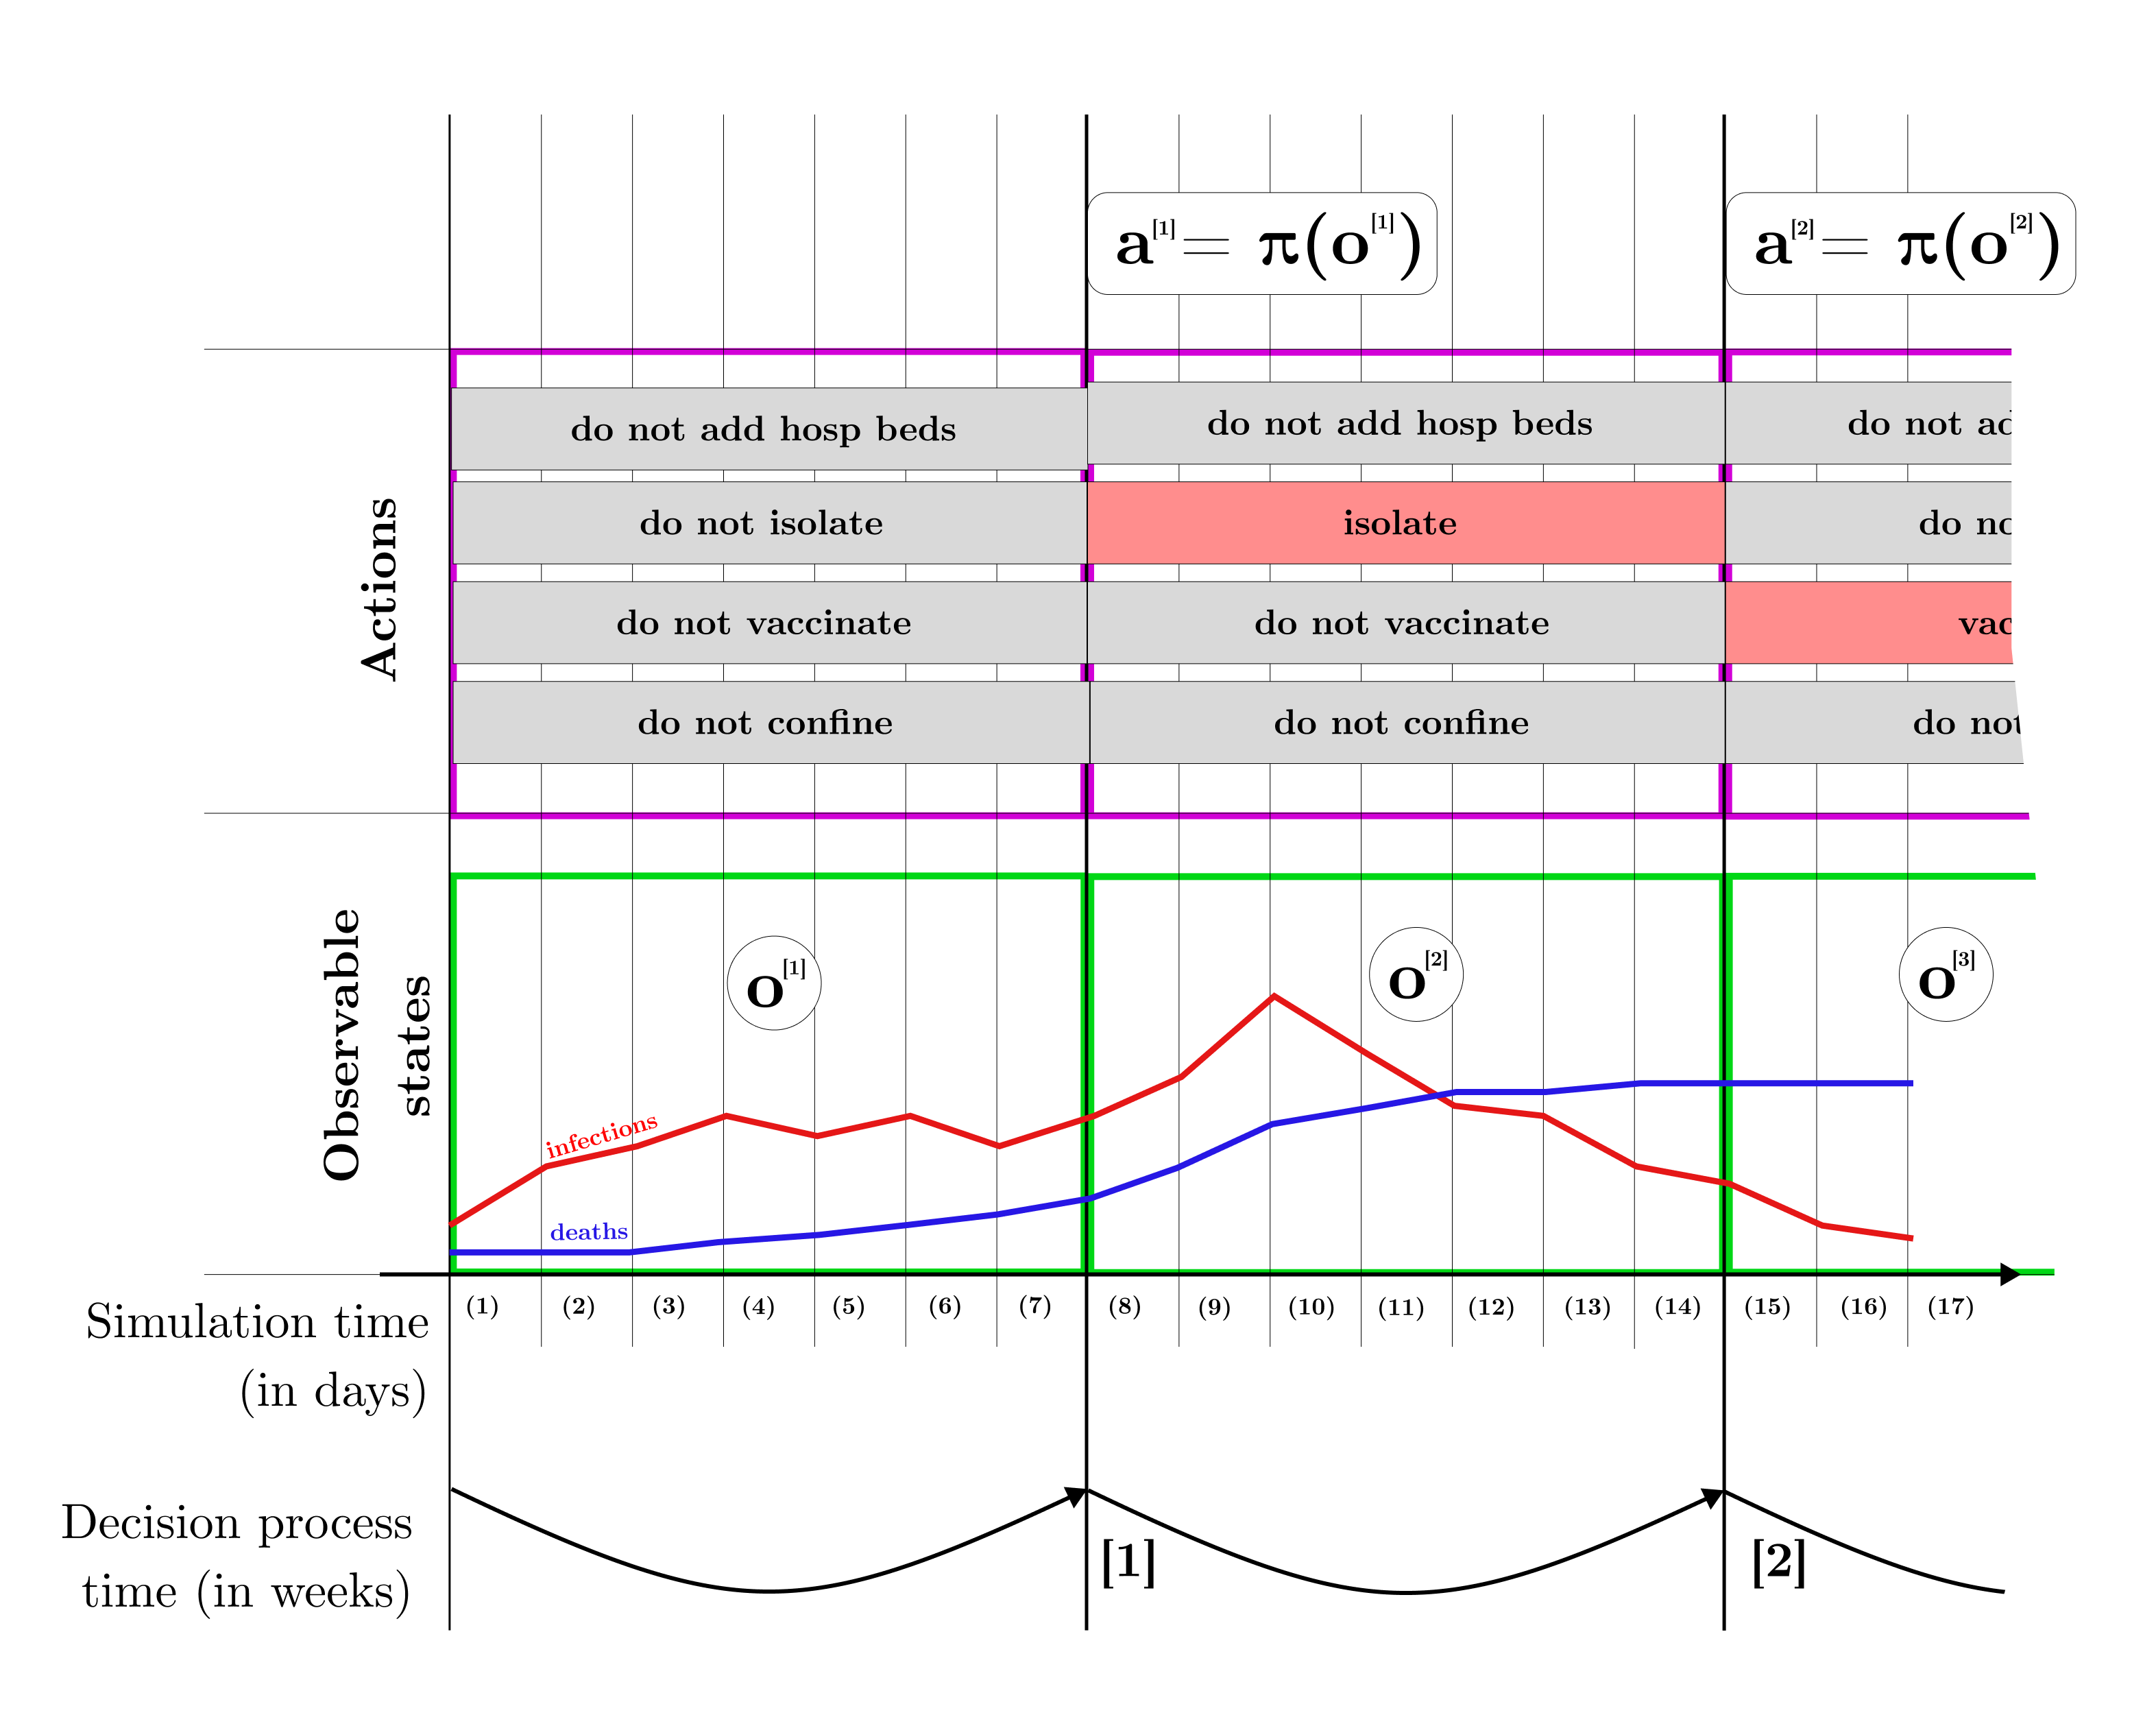
\includegraphics[width=0.6\textwidth]{figures/POMDP.png}
    \caption{Illustration of part of a decision process episode. Note the difference between simulation time (in days) and decision process step (in weeks), as well as the fact that actions are always taken based on an observation from the previous week. For instance, on week $1$, the agent makes observation $\mathbf{o}^{[1]}$, and uses it to compute action $\mathbf{aË}^{[1]}$, which is applied until the end of week $2$. }
    \label{fig:pomdp}
\end{figure}

\subsubsection*{The environment}

The decision process takes place during $30$ week \textbf{episodes} (an episode therefore lasts $310$ days).
For each episode, the model is initialized with every person in the \textit{susceptible} state except for a very small subset of randomly contaminated individuals. The process advances one week at a time. At the end of each week the agent gets an observation $\mathbf{o}^{[w]}$ and takes an action $\mathbf{a}^{[w]}$. As is most commonly the case, we call \textbf{policy} the function $\pi : O \rightarrow A$ that maps observations to actions. See figure \ref{fig:pomdp}.


\subsection*{The reward}

\begin{table}[ht]
  \begin{center}
    \begin{tabular}{||l | l ||} 
     \hline
     Term & Value Represented  \\ [0.5ex] 
     \hline\hline
     $R_\text{c}$ & constant positive reward term.  \\ 
     \hline
     $D$ & cost of deaths. \\ 
     \hline
     $V$ & cost of vaccination. \\ 
     \hline
     $H$ & cost of extra hospitalization. \\ 
     \hline
     $C$ & cost of confinement. \\ 
     \hline
     $I$ & cost of isolation.  \\ 
     \hline
     $ \mathbf{1}_{vac} ,\mathbf{1}_{hosp},\mathbf{1}_{conf},\mathbf{1}_{isol}$ & indicator functions for vaccination, hospitalization, confinement and isolation.  \\ 
      & I.e.  $\mathbf{1}_{action} = 1$ if the action is take, $0$ otherwise. \\ 
     \hline
     $ \mathbf{1}_{vac}^+,\mathbf{1}_{isol}^+,\mathbf{1}_{conf}^+$ & indicator functions for transition to vaccination, isolation or confinement.  \\ 
     & I.e.  $\mathbf{1}_{action}^+ = 1$ if the action was just taken, $0$ otherwise. \\ 
     \hline
     $\Delta d_\text{city}^{(d)} =  d_\text{city}^{(d)} -  d_\text{city}^{(t-1)}$ & new deaths from one timestep to the next.  \\ 
     \hline
    \end{tabular}
    \end{center}
    \caption{Terms of the reward function.}
    \label{table:reward}
\end{table}


In order to better quantify the performance of a policy we decide to compute a metric of the performance of a given policy.
Because we are going to train reinforcement learning agents to maximize this metric we call it a reward. We define the reward as:

\begin{equation}
    R^{[w]} =  R_\text{c}
    - \mathcal{C}(\mathbf{a}^{[w]})
    - D \cdot \Delta d_\text{total}^{[w]}
\end{equation}
which is split into three terms: a \textit{constant reward} term $R_\text{c}$ to which we subtract two costs, a death cost $D \cdot \Delta d_\text{total}^{[w]}$ which is directly proportional to the number of people who died since the last POMDP step, and an action cost $\mathcal{C}(\mathbf{a}^{[w]})$. The action cost itself consists in fixed cost associated with taking each action for one time step  (the price of vaccines in the case of vaccination) to which we add a cost for announcing that an action moves from \texttt{False} to \texttt{True} at a given time step. This is meant to model the additional cost that comes with the transition to a new policy (for instance the extra cost induced when setting up new vaccination center), and to encourage convergence to a less noisy policy.

\begin{equation}
  \begin{aligned}
    \textbf{Action cost} &&
    \mathcal{C}(\mathbf{a}^{[w]}) =  
    \mathcal{A}(\mathbf{a}^{[w]}) 
    + \mathbf{1}_{vac}  \cdot V
    + \mathbf{1}_{hosp} \cdot H
    + \mathbf{1}_{conf} \cdot C
    + \mathbf{1}_{isol} \cdot I \\
    \textbf{Annoucement costs} &&
    \mathcal{A}(\mathbf{a}^{[w]})  = A \cdot (\mathbf{1}^+_\text{vac} + \mathbf{1}^+_\text{isol} + \mathbf{1}^+_\text{conf})
  \end{aligned}
\end{equation}
\noindent
all the terms of the rewards are detailled in the table \ref{table:reward}. 




\subsection*{Question 1.a) study the behavior of the model when epidemics are unmitigated}

Run the epidemic simulation for \textit{one episode} ($30$ weeks), \textit{without epidemic mitigation} (meaning no action is taken, i.e. all values in the action dictionary are set to \texttt{False}) and \textbf{produce three plots}:
\begin{enumerate}
  \item A plot of variables $s_\text{total}^{[w]},e_\text{total}^{[w]},i_\text{total}^{[w]},r_\text{total}^{[w]},d_\text{total}^{[w]}$ over time, where time is measured in weeks and all the variables share the $y$ axis scaling.
  \item A plot of variables $i_\text{total}^{[w]},d_\text{total}^{[w]}$ over time, where time is measured in weeks and all the variables share the $y$ axis scaling.
  \item A set of plots of variables $i_\text{city}^{[w]},d_\text{city}^{[w]}$ over time, where time is measured in weeks (one subplot per-city, variables share the $y$-scaling per-city).
\end{enumerate}
\textbf{Discuss the evolution of the variables over time.}

\section{Professor Russo's Policy}

Since the epidemic hit Listenburg before Switzerland, the listenburgish medical community has had time to study the epidemic behavior of the disease and one of the listenburgish experts, professor Russo, suggests the following mitigation policy:

\begin{algorithm}[H]
    \SetAlgoLined
    \caption{Pr. Russo's Policy ($\pi_\text{Russo}$)}
    \textbf{Input : } $x \leftarrow i_\text{total}^{[w]}$ number of infected people at the end of week $w$\\
    \If(){$x > 20'000$}{
      \textit{Confine the entire country for 4 weeks}
    }
\end{algorithm}
The number of infected cases is not evaluated during a confinement period, \emph{i.e.} if the policy declares a 4-week
confinement starting at week $w$ and the number of infected people is still $> 20'000$ at week $w+2$, a new 4-week
confinement does not start at $w+2$.

\subsection*{}

\subsection*{Question 2.a) Implement Pr. Russo's Policy}

Implement Pr. Russo's Policy \textbf{as a python class} (\textit{we recommend that you subclass the \texttt{Agent} abstract class provided with the project files, and as is demonstrated in the tutorial notebook}). Run the epidemic simulation for one episode using Pr. Russo's Policy to pick actions and \textbf{produce four plots}:
\begin{enumerate}
  \item A plot of variables $s_\text{total}^{[w]},e_\text{total}^{[w]},i_\text{total}^{[w]},r_\text{total}^{[w]},d_\text{total}^{[w]}$ over time, where time is measured in weeks and all the variables share the $y$ axis scaling.
  \item A plot of variables $i_\text{total}^{[w]},d_\text{total}^{[w]}$ over time, where time is measured in weeks and all the variables share the $y$ axis scaling.
  \item A set of plots of variables $i_\text{city}^{[w]},d_\text{city}^{[w]}$ over time, where time is measured in weeks (one subplot per-city, variables share the $y$-scaling per-city).
  \item A plot of the action taken by the policy over time (whether the policy chooses to confine or not).
\end{enumerate}

Discuss how the epidemic simulation responds to Pr. Russo's Policy (focus on how it differs from the unmitigated scenario).


\subsection*{Question 2.b) Evaluate Pr. Russo's Policy}

In order to be able to make meaningful conclusions about the behavior of the policy, you will need properly evaluate its behavior.
To do so, running a single episode is not enough. \textbf{Implement the following evaluation procedure}: run $50$ simulation episodes where actions are chosen from policy $\pi$ (in this case $\pi$ will be $\pi_\text{Russo}$, but you should make the effort to write evaluation code in which you can easily change the policy being evaluated as you will be asked to evaluate each policy you train later). \textbf{For each episode, save the following values}:
\begin{enumerate}
  \item the \textbf{number of total confined days} $N_\text{confinement}=7\cdot \text{ number of confined weeks }$,
  \item the \textbf{cumulative reward} (the sum of all rewards collected during the episode) $R_\text{cumulative} = \sum_{i \in [0 , ..., 30]} R^{[i]}$.
  \item the \textbf{number of total deaths} $N_\text{deaths} = d_\text{total}^{[30]}$,
\end{enumerate}
\textcolor{MidnightBlue}{Make sure to always be using the same sequence of random seeds (see the \textbf{tutorial notebook} for details on the environment seed) when evaluating different policies, in order to ensure that results are repoducible. (To check that they are, run the eval twice, and check that you get the same average values).} Once those values are logged for each episode, \textbf{plot a histogram}. \textcolor{MidnightBlue}{(Use the histogram plotting function from the tutorial notebook.)}
  
\section{A Deep Q-learning approach}

Now you will try to improve on Pr. Russo's Policy using Deep-Q-Learning. In the following section you will implement a first version of Deep-$Q$-learning with a simple action space.\\

The method that you will implement is the Deep Q-Network (DQN) algorithm, as first presented in \href{https://arxiv.org/pdf/1312.5602.pdf}{Mnih et. al 2013}. We recommend that you implement the algorithm using the \textit{pytorch} library and that you make use of \href{https://pytorch.org/tutorials/intermediate/reinforcement_q_learning.html}{the \textit{pytorch} example for DQN} which is a really good reference implementation. \\

Note unless special measures are taken, the training of neural networks is non-deterministic in most deep-learning libraries.
To ensure that your results are reproducible you will thus need to seed not only the environment but also your deep-learning library.
Refer to the \textbf{jupyter tutorial notebook} for instructions.\\


For each deep-learning policy that you train in this project we recommend that you use the following hyperparameters.
If you wish so, you are free to test other values, but as searching through the hyperparameter-space can be quite a tedious experience we are giving you values that we know will allow the algorithm to converge to a good policy.

\noindent
\textbf{Remark on pre-processing: }note that if you "naively" scale the observations, you will end up with really small values in the observation tensor (since the number of deaths is much smaller than the total population).
To avoid this, we recommend that you pass the (scaled) observations through a $(\cdot)^{\frac{1}{4}}$ function.

\begin{table}[ht]
\begin{center}
  \resizebox{\columnwidth}{!}{
  \begin{tabular}{||c | l ||} 
  \hline
  hyperparameter & Value  \\ [0.7ex] 
  \hline\hline
  neural network architecture & A $3$ hidden layer fully connected neural net with layers of size  $\textbf{input size}, ~ 64,~ 32,~ 16,~\textbf{output size}$  (see figure \ref{fig:arch})\\ 
  \hline
  activations & ReLU activations after each layers (except the output which is purely linear) \\ 
  \hline
  target update rate & (fully) update the target network every $5$ episodes \\
  \hline
  training length & train for $500$ episodes \\ 
  \hline
  learning rate & $5 \cdot 10^{-3}$ (when the action-space is  binary)\\ 
  \hline
  discount factor $\gamma$ & $0.9$ \\ 
  \hline
  buffer size & $20000$ \\ 
  \hline
  batch size & $2048$ \\ 
  \hline
  \end{tabular}
  }
  \end{center}
  \caption{Suggested training hyperparameters.}
  \label{table:hyperparameters}
\end{table}

% \textbf{\textcolor{BrickRed}{Guideline : log the loss and Q-values for debug and analysis purposes}}


\begin{figure}[h!]
  \centering
  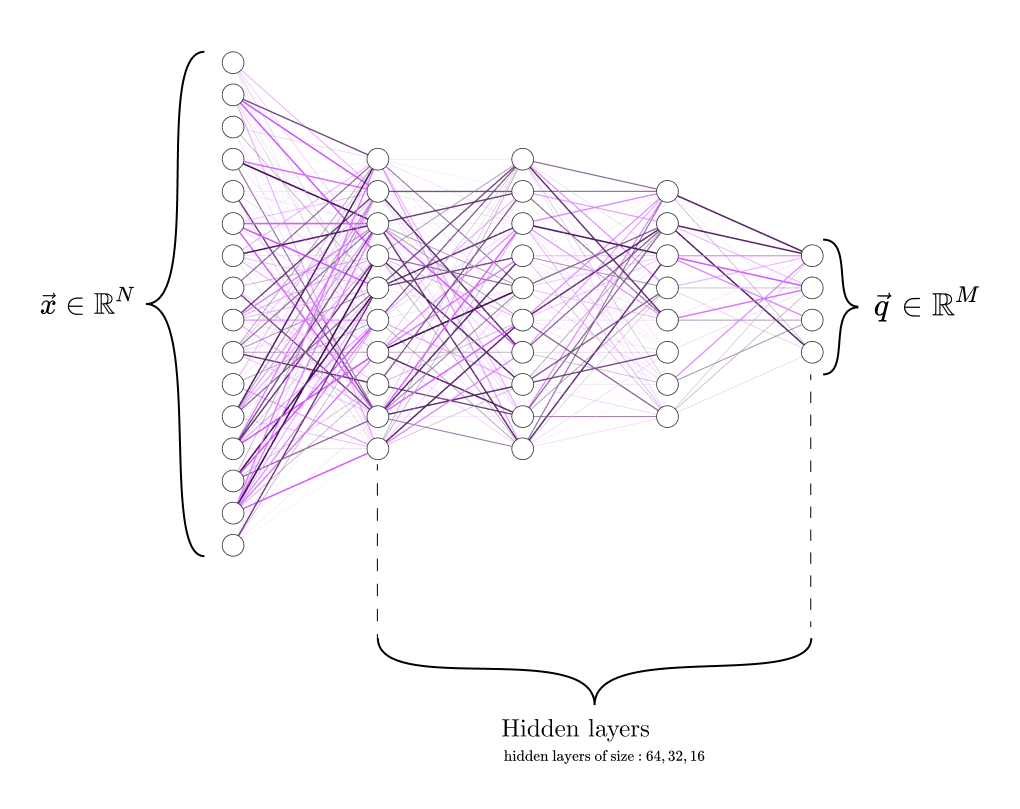
\includegraphics[width=.7\textwidth]{figures/arch.png}
  \caption{Network architecture.}
  \label{fig:arch}
\end{figure}

\subsection{Deep Q-Learning with a binary action space}

Your friend suggests using Deep Q-learning as an improvement to Pr. Russo's policy, using a very simple action/observation-space. \textit{The action space is binary} (meaning the neural network has an output size of $2$: where one neuron estimates the $Q$ value of confinement, and the other the Q-value of non confinement). The \textit{observation space} contains the measurement of the proportion of dead and infected people in each city, each day of a given week (it is a matrix of shape $2 \times 9 \times 7$, exactly as in figure \ref{fig:obs}).

\subsection*{Question 3.a) implementing Deep Q-Learning}
Implement and train the Deep Q-Learning agent $\pi_\text{DQN}$ for $500$ training episodes, with $\epsilon=0.7$. \textbf{For each episode, log the cumulative reward.}
You will see that Deep Q-Learning training curves are quite noisy, so to better evaluate the learning process we ask you to \textbf{implement the following evaluation procedure}.


\begin{algorithm}[H]
  \SetAlgoLined
  \caption{Training/Logging procedure for DQN}
  \For{episode in 500}{
    Run an episode. \\
    Log the cumulative reward $R_\text{cumulative}$ to \textit{training trace}. \\
    Run a training step. \\
    \If(){$\text{episode} \% 50 = 0$ or $\text{episode}=500$}{
      Run a $20$ episode evaluation procedure, log their cumulative rewards. \\
      Compute the average cumulative reward over the $20$ evaluation episodes and log it to \textit{eval trace}.
    }
    
  }
\end{algorithm}

\noindent
The total training time is $500$ episodes. Every $50$ episodes, run a $20$ episode evaluation process \textit{with $\epsilon=0$  (no exploration) and no learning occurring} and compute an average cumulative reward across the $20$ episodes.
We call the plot of the training reward, the \textit{training trace} and the plot of the evaluation reward the \textit{evaluation trace}.
\textcolor{MidnightBlue}{For the evaluation procedure before, be careful to always use the same seed, to ensure repoducible results.} Once you have successfully done so, \textbf{plot the training trace} and the \textbf{eval trace}.
(We expect a plot of the reward in $y$ and the training episode in $x$ both for the training trace and the eval trace).
It might be more readable to plot the training trace as a scatter plot.
Since training results can be hard to reproduce, \textbf{we ask you to average the eval trace across three full training processes (for the training trace, you can just scatter-polt the three trainings together).}
Do not forget to \textbf{save your trained weights} (the ones which gave the best reward on evaluation) for later evaluation.
\textbf{Does your agent learn a meaningful policy?}
\textbf{Record three example episodes} where actions are picked by the best policy $\pi^*_\text{DQN}$ you obtain.
\textbf{Plot one of those episodes}, using the same plotting procedure as in question \textit{2.a)} and \textbf{interpret the policy}.

\subsection*{Question 3.b) decreasing exploration}
Implement and train Deep Q-Learning agent for $500$ training episodes with decreasing $\epsilon$:
\begin{align}
  \epsilon(t)= \max\left(\frac{\epsilon_0(T_\text{max} - t)}{T_\text{max}}, \epsilon_\text{min}\right)
\end{align}
where $t$ is the episode number, $T_\text{max}=500$, $\epsilon_0 = 0.7$ and $\epsilon_\text{min} = 0.2$. \textbf{Plot the evaluation and training traces} on a shared plot with the traces from question \textit{3.b)}, (we ask you to average across $3$ training runs). \textbf{Compare and discuss the results} between questions 3.a) and 3.b). \textbf{Which policy gets the best results and why?}



\subsection*{Question 3.c) evaluate the best performing policy against Pr. Russo's policy}

Run the best performing policy $\pi^*_\text{DQN}$ through the evaluation code that you wrote to evaluate Pr. Russo's policy in question 2.b), \textbf{generate the same histogram plots and compare the results}. \textbf{Did the reinforcement learning policy outperform Pr. Russo'}s, if so in what sense?  

\section{Dealing with a more complex action Space}

From here on, we expect that all agents are trained with decreasing exploration (following the same $\epsilon(t)$ as described in question 3.b). \\

In order to achieve stable training, \textbf{the multi-action policies trained in question \textit{4.1} and \textit{4.2} require that learning rate to be much smaller than in the binary action situation}. \textbf{We recommend that you use a learning rate $\text{lr} = 10^{-5}$.}

\subsection{Toggle-action-space multi-action agent}


\begin{figure}[h!]
    \centering
    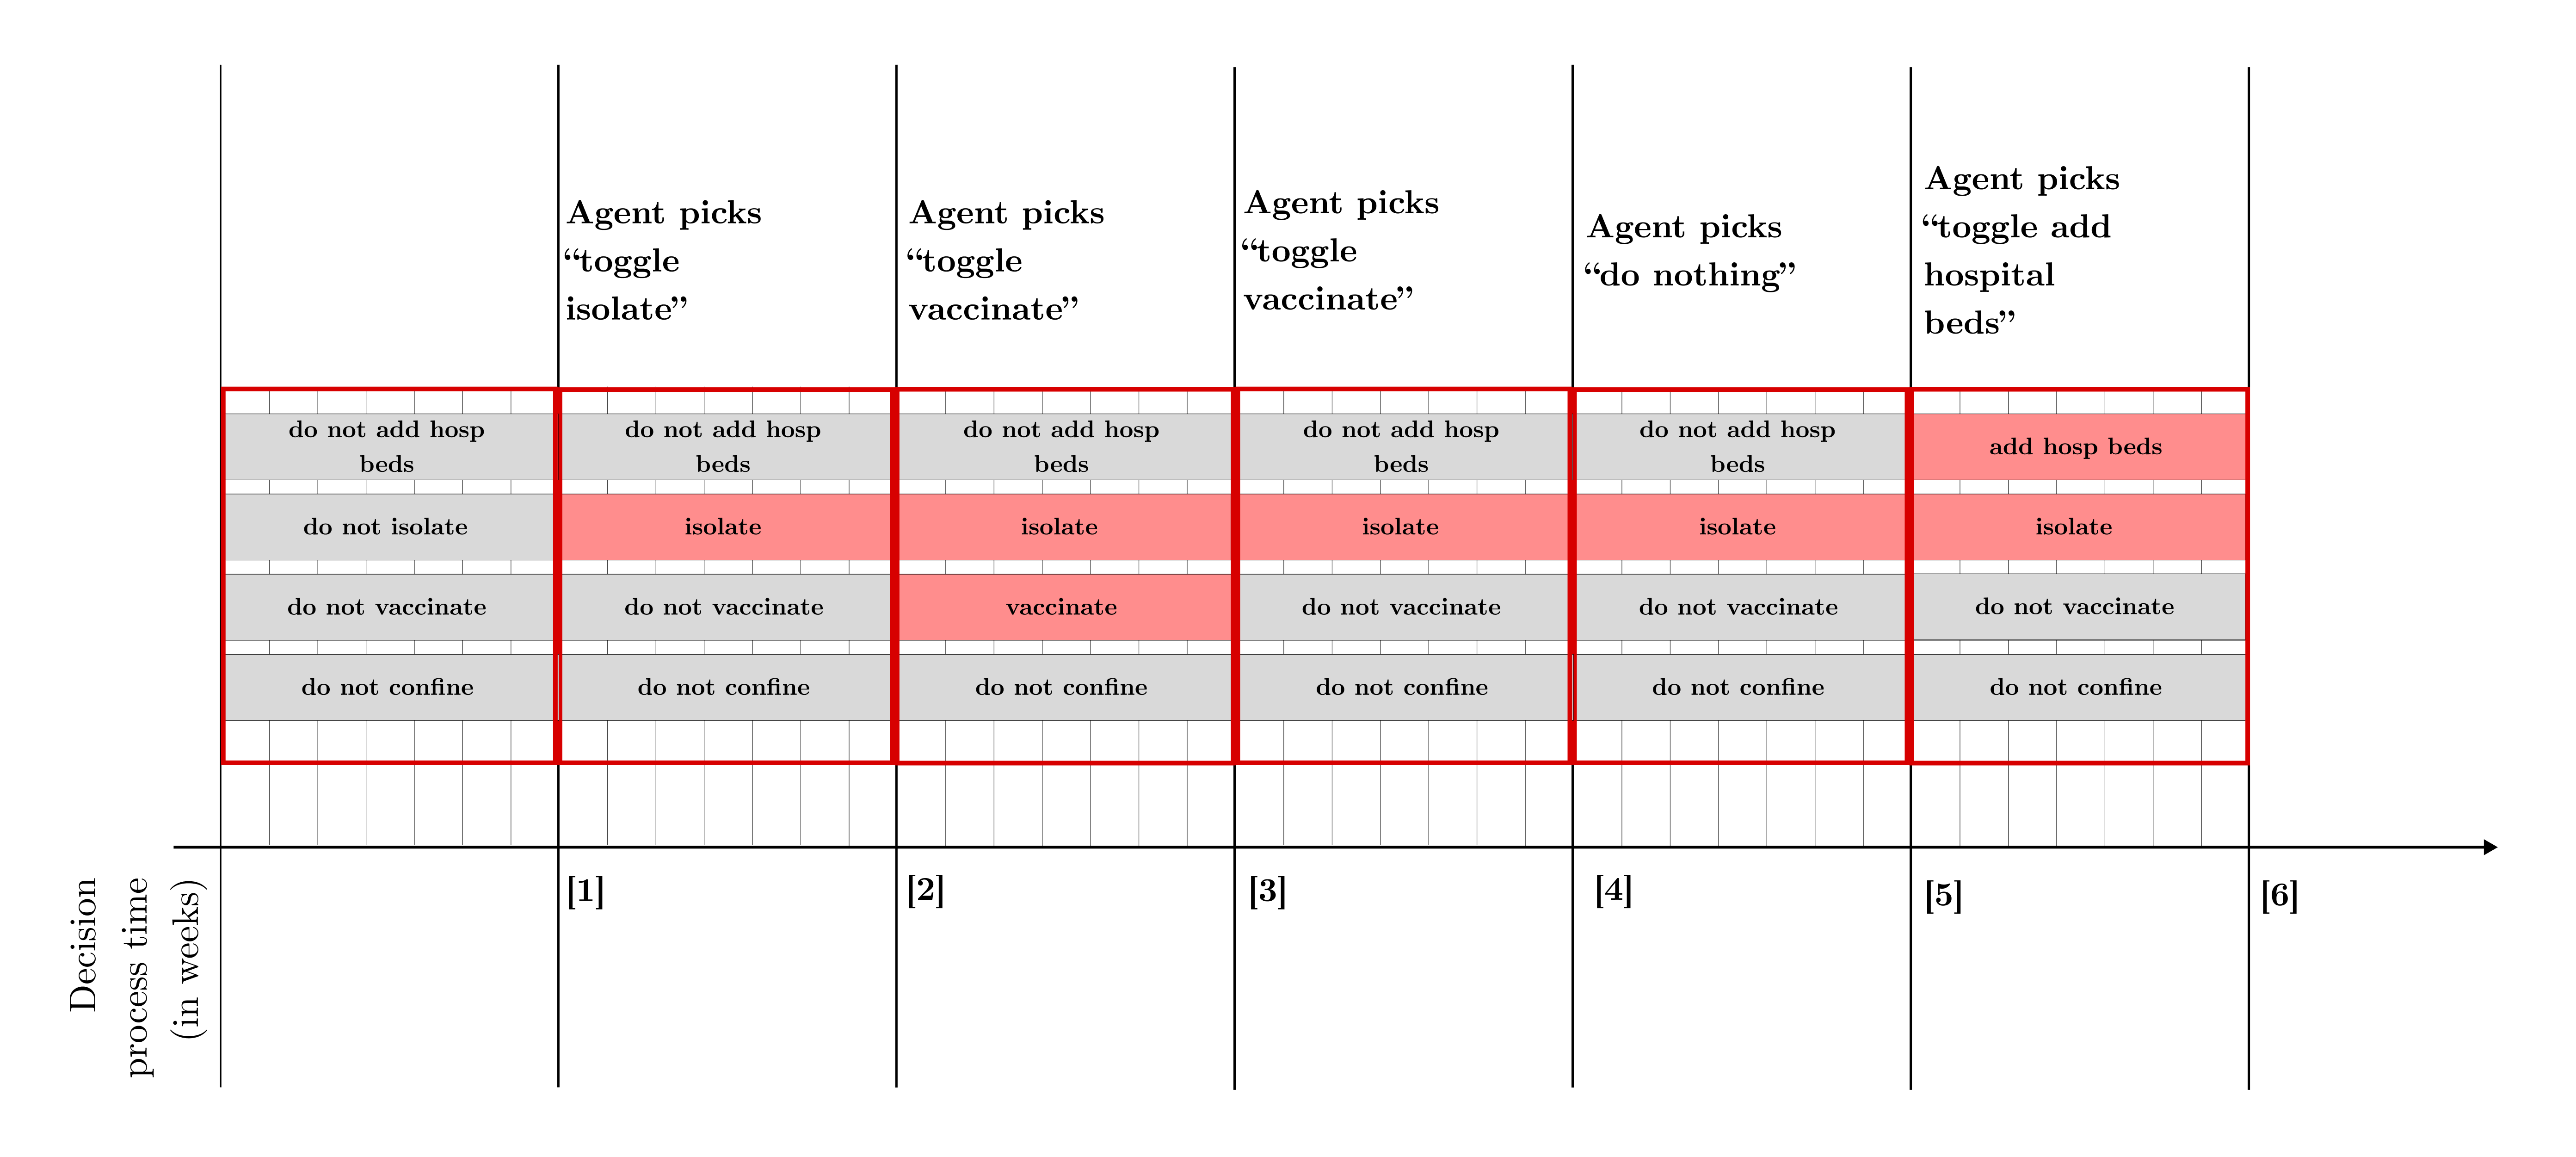
\includegraphics[width=\textwidth]{figures/toggle.png}
    \caption{Example decision process with the toggled action space.}
    \label{fig:toggle}
\end{figure}

In order to to allow your agent to be use every action in the environment, your Friend proposes the following method. Let the action space have $5$ actions: [\texttt{do nothing},\texttt{toggle confinement},\texttt{toggle isolation}, \texttt{toggle additional hospital beds}, \texttt{toggle vaccination}]. When the agent takes a \texttt{toggle} action, the state of that specific action changes state from what is previously was to the opposite. If the agent takes the \texttt{does nothing} action, no action is changed.
For instance if the current state of the \textit{isolation} action is \texttt{True}, picking the action \texttt{toggle isolation} makes the state of the action \texttt{False} in the next \textit{POMDP step} (see figure \ref{fig:toggle} for an example). 
For each of the $5$ actions, a Q-value is estimated.
Because the agent doesn't have direct control anymore, and because the $Q$-value of the \textit{toggle} actions changes
depending on whether their state is set to \texttt{True} or \texttt{False}, we also need to change the observation space
to include the current state of each action as an observation. This should be implemented using action and observation preprocessors, as is displayed in the tutorial notebook.

\subsubsection*{Question 4.1.a) (Theory) Action space design}
Why would one want to use such an action-observation space as the one above, rather than directly compute $Q(s,a)$ for each action? \textbf{Discuss, the impact on network architecture and on training.} 
\subsubsection*{Question 4.1.b) Toggle-action-space multi-action policy training}
Implement the toggled-action and observation spaces and train your Deep Q-Learning agent on it. We call the best trained policy on this action-space $\pi^*_\text{toggle}$. \textbf{Plot the training and evaluation traces} (we ask you to average across $3$ training runs). \textbf{Is the agent properly learning?} Run a $3$ episodes of the best policy $\pi^*_\text{Toggle}$, to better understand the behavior of the learned policy.  \textbf{Plot one of those episodes and interpret the policy}.

\subsubsection*{Question 4.1.c) Toggle-action-space multi-action policy evaluation}
Evaluate the $\pi^*_\text{Toggle}$ policy trained in question \textit{4.1.b)}, using the evaluation procedure that you previously defined.
\textbf{Plot the histograms} and discuss the results.
\textbf{How does the policy perform compared to the binary action policy} evaluated in question 3.c?

\subsubsection*{Question 4.1.d) (Theory) question about toggled-action-space policy, what assumption does it make?}

In question \textit{4.1.b)}, you implemented a toggle-action-space policy.
\textbf{What assumptions does the use of such a technique make on the action space}?
Could you \textbf{think of an action space for which toggling the actions would not be suitable}? Discuss.

\subsection{Factorized Q-values, multi-action agent}

% \begin{figure}[h!]
%     \centering
%     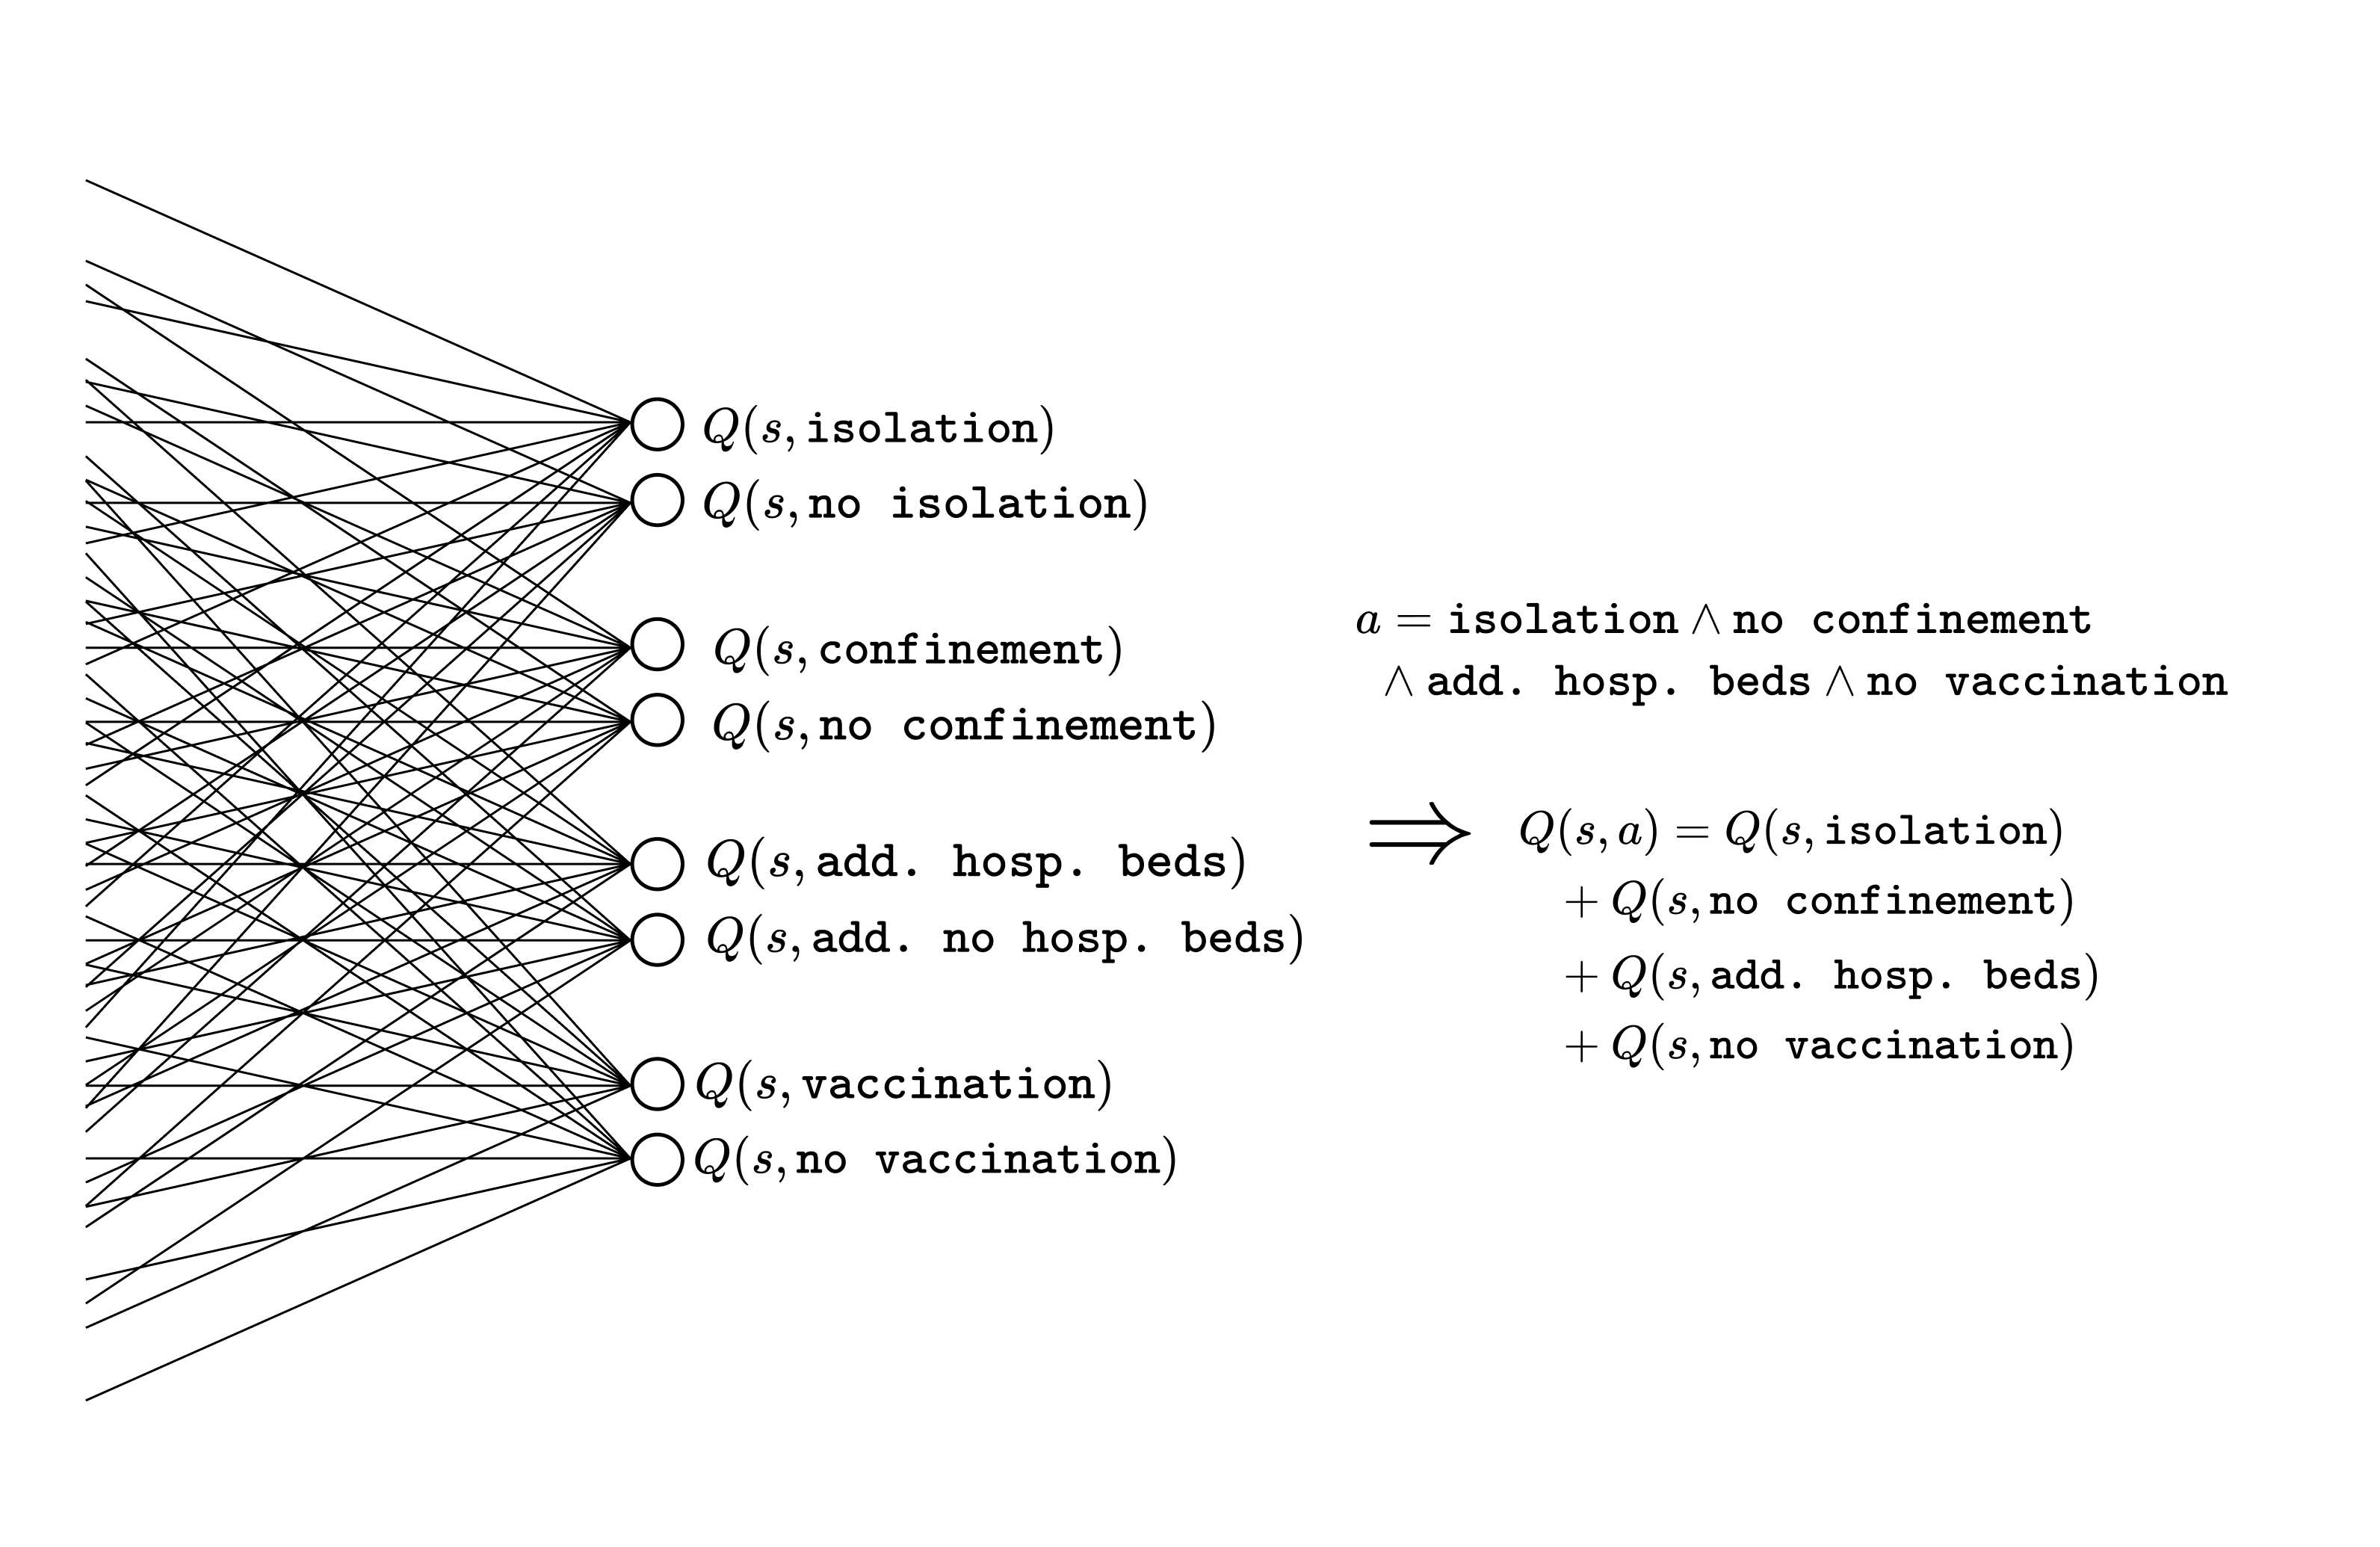
\includegraphics[width=0.6\textwidth]{figures/Factor.png}
%     \caption{Illustration of the factorization performed to train in the factorized-$Q$-value setting.}
% \end{figure}

You decide to try an alternative approach, \textit{factorized Q-values}. Instead of implementing a toggled behavior as above you let the neural network decide whether to make each decision \texttt{True} or \texttt{False} independently. To do so you create a $4\times 2$ output layer for your Deep Q Network. Each decision ($a_\text{conf} = \texttt{True}$ or $a_\text{conf} = \texttt{False}$, $a_\text{isol} = \texttt{True}$ or $a_\text{isol} = \texttt{False}$, etc.) is associated with a neuron pair. The $Q$-value of the complete action is given by the sum of the $Q$-values of each decision picked:
\begin{equation}
  Q(\mathbf{a}^{[w]}, s) = Q(  a_\textit{conf}^{[w]} \cup a_\text{isol}^{[w]} \cup a_\text{hosp}^{[w]} \cup a_\text{vacc}^{[w]} , s) = \sum_{\mathfrak{d} \in \text{decisions}} Q(a_\mathfrak{d},s).
\end{equation}
In other words it is a sum of half the neurons of the last layer, where we choose each neuron according to which decision was made. Once $Q$-values are picked in that fashion we get that:
\begin{equation}
\begin{aligned}
  \text{argmax}_{ \mathbf{a}^{[w]} }  Q(\mathbf{a}^{[w]},s) = \text{argmax}_{ \mathbf{a}^{[w]} } \sum_{\mathfrak{d} \in \text{decisions}} Q(a_\mathfrak{d},s) \\
  = \bigcup_{\mathfrak{d} \in \text{actions}}  \text{argmax}_{  a_\mathfrak{d}^{[w]} }  Q(a_\mathfrak{d}^{[w]},s)
\end{aligned}
\end{equation}
\noindent
I.e. we can pick pick the decision that maximizes the $Q$-value term associated with a given action for each element.
We then train our neural network by backpropagating on the sum of whatever actions we independently picked.
Since there is no toggle behavior anymore, you can use the same observation space as in question \textit{3.a)}
(no need to expand the observation space in any specific way).
You can use the MultiBinary space type to create the action space.\\

\subsubsection*{Question 4.2.a) multi-action factorized Q-values policy training}
Implement the multi-action factorized Q-values agent and observation spaces and \textbf{train your Deep Q-Learning agent on it}.
We call the best-performing trained agent $\pi_\text{factor}^*$.
\textbf{Plot the evaluation and training traces} on a graph together with the traces from the toggle-action-space training (averaged across $3$ training runs).
\textbf{Does it successfully learn?}
Run a few episodes of the best policy $\pi^*_\text{factor}$, to better understand the behavior of the learned policy.
\textbf{Plot one of those episodes and interpret the policy}. Is the policy realistic?


\subsubsection*{Question 4.2.b) multi-action factorized Q-values policy evaluation}
Evaluate the best policy ($\pi_\text{Factor}^*$) trained in question \textit{4.2.a)}, using the evaluation procedure that you previously defined. \textbf{Plot the histograms}, discuss the results, and compare them to the policy implemented in \textit{4.1.b)}. \textbf{How does it compare to the toggled policy}?


\subsubsection*{Question 4.2.c) (Theory) Factorized-Q-values, what assumption does it make?}

In question \textit{4.2.a)}, you implemented a factorized-Q-value policy.
\textbf{What assumptions does the use of such a technique make on the action space?}
Could you \textbf{think of an action space for which factorizing Q-values would not be suitable}? Discuss.

\section{Wrapping Up}

\subsubsection*{Question 5.a) (Result analysis) Comparing the training behaviors}

Compare the evaluations and training curves of \textbf{Pr. Russo's Policy}, \textbf{single-action DQN}, \textbf{factorized Q-values} and \textbf{toggled-action-space} policies. Discuss the performance differences, what do you observe? How do the two approaches compare ? What approach performs best? Why?

\subsubsection*{Question 5.b) (Result analysis) Comparing policies}
Run the evaluation procedure with each ( $\pi_\text{DQN}$, $\pi_\text{toggle}$, $\pi_\text{factor}$ as well as the original $\pi_\text{russo}$) trained policy (always pick the best-performing policy) for $50$ episode and compute the following metrics (all of the averages are empirical means computed over the $50$ episodes):
\begin{enumerate}
  \item the average number of \textbf{total confined days} $\text{avg}[N_\text{confinement}]$ (\textit{lower is better}),
  \item the average number of \textbf{total isolation days} $\text{avg}[N_\text{isolation}]$ (\textit{lower is better}),
  \item the average number of \textbf{total vaccination days} $\text{avg}[N_\text{vaccination}]$ (\textit{lower is better}),
  \item the average number of \textbf{total additional hospital bed days} $\text{avg}[N_\text{confinement}]$ (\textit{lower is better}),
  \item the average \textbf{number of total deaths} $\text{avg}[N_\text{deaths}]$ (\textit{lower is better}),
  \item the average \textbf{cumulative reward} $\text{avg}[R_\text{cumulative}]$ (\textit{higer is better}).
\end{enumerate}
\noindent
Make a table with each of those values for each policy. Clearly mark the best performing policy with respect to each metric. Exclude the policies that do not have access to an action from the relevant metric (for instance, as $\pi_\text{Russo}$ does not have access to vaccination, exclude it from the total vaccination days comparaison). Discuss.

\subsubsection*{Question 5.c) (Interpretability) Q-values}
For both $\pi_\text{DQN}$ and $\pi_\text{factor}$, produce a plot for visualizing the estimated $Q$-values for one episode. \textbf{Run a simulation episode, and plot a heat-map of the evolution of all $Q$-values with time}, with action selections in the $y$-axis and time (in weeks) in the $x$ axis. Clearly label which action is associated with which $Q$-value on the $y$ axis as well as the evolution of time in weeks, provide a color-bar. \textbf{Discuss your results.} How interpretable is your policy?

\subsubsection*{Question 5.d) (Theory), Is cumulative reward an increasing function of the number of actions?}
In the following project you have implemented different policies acting on the exact same environment with a different number of actions.
\textbf{Is cumulative reward an increasing function of the number of actions?} (\textit{In other words, does adding an action always yield a better reward?})



\end{document}